
\documentclass[runningheads]{llncs}

\usepackage{graphicx}
\usepackage{booktabs}
\usepackage{multicol}

\begin{document}
%
\title{Data Mining 1: \\
Predicting positions of soccer players  \\
Project Report}


\vspace{2cm}
\author{Team No. 9\\
\vspace{1cm}
presented by\\
Jurgen Amedani (1628022), Cara Maria Damm (1631263), Paul Hesselmann (1371380), Allwyn Menezes (1671634), Martin Mlinac (1364487), Carmen Rannefeld (1631070)\\
\vspace{1cm}
submitted to the \\
Data and Web Science Group\\
Prof. Dr. Bizer\\
University of Mannheim}

\institute{}
\maketitle              % typeset the header of the contribution
\newpage
%1. What is the problem you are solving?
\section{Application Area and Goals}
\section{Structure and Size of Data}
In this project, which focusses on soccer analytics, the FIFA 19 dataset from kaeggle is used. It includes information about every player who is registered to the sofifa database \cite{ref_sofifa}. 
The database includes more than 18207 registered players, for each player 86 different attributes are available. The attributes can be grouped in the following 10 groups: 
\begin{multicols}{2}
	\begin{enumerate}
	\item Personal information
	\item Contract Information
	\item Mental Capabilities
	\item Sports and Soccer Statistics
	\item Attacking Statistics  
	\item Skill Statistics
	\item Defending Statistics
	\item Movement Statistics
	\item Goalkeeping Statistics
\item Strength Statistics
\end{enumerate}
\end{multicols}

The table below contains the attributes for each group:

\setlength{\columnseprule}{0.4pt}
\begin{multicols}{3}
\begin{itemize}
\item	Personal information
\begin{itemize}
\item	Database ID
\item	Name
\item	Age
\item	Nationality
\item	Height 
\item	Weight
\end{itemize}
\item	Contract Information
\begin{itemize}
\item	Club
\item	Wage
\item	Release Clause
\item	Jersey Number
\item	Joined date
\item	Loaned from
\item	Contract valid until
\end{itemize}
\item	Mentality Statistics
\begin{itemize}
\item	Aggression
\item	Interceptions
\item	Positioning
\item	Vision
\item	Penalties
\item	Composure
\columnbreak
\end{itemize}
\item	Sports and Football information
\begin{itemize}
\item	Value 
\item	International Reputation
\item	Overall Ranking
\item	Potential (correlation to overall ranking)
\item	Special 
\item	Position (club)
\item	Position (national team)
\item	Preferred Foot
\item	Week Foot
\item	Skill Moves
\item	Work Rate Defense
\item	Work Rate Attack 
\item	Body Type 
\item	Real Face 
\end{itemize}
\item	Attacking Statistics
\begin{itemize}
\item	Crossing
\item	Finished
\item	Heading Accuracy
\item	Short Passing
\item	Volleys
\end{itemize}
\columnbreak
\item	Skill Statistics
\begin{itemize}
\item	Dribbling
\item	Curve
\item	Free Kick Accuracy
\item	Long Passing
\item	Ball Control
\end{itemize}
\item	Defending Statistics
\begin{itemize}
\item	Marking
\item	Standing Tackle
\item	Sliding Tackle
\end{itemize}
\item	Movement Statistics
\begin{itemize}
\item	Acceleration
\item	Sprint Speed
\item	Agility
\item	Reactions
\item	Balance
\end{itemize}
\item	Goalkeeping Statistics
\begin{itemize}
\item	GK Diving
\item	GK Handling
\item	GK Kicking
\item	GK Positioning
\item	GK Reflexes
\end{itemize}
\item	Power Statistics
\begin{itemize}
\item	Shot Power
\item	Jumping
\item	Stamina
\item	Strength
\item	Long Shots
\end{itemize}
\end{itemize}
\end{multicols}

In the dataset one player is assigned to exactly one position out of 25 available positions. As players might play on different positions during a season or training, the potential for 24 positions (except goalkeeper position) is recognized as well in the dataset. The position is written down as abbreviation meaning:
\setlength{\columnseprule}{0.4pt}
\begin{multicols}{3}
\begin{itemize}
\item	Forwards:
\begin{itemize}
\item	RF Right forward
\item	CF Center forward
\item	LF Left forward
\item	RS Right Striker
\item	ST Striker
\item	LS Left Striker
\item	RW Right wing
\item	LW Left wing 
\end{itemize}
\item	Midfielders:
\begin{itemize}
\item	LAM Left attacking midfield
\item	RAM Right attacking midfield
\item	CAM Center attacking midfield
\item	LM Left midfield
\item	CM central midfield
\item	LCM Left center midfield
\item	RCM Right center midfield
\item	RM Right midfield
\item	LDM Left defensive midfield
\item	CDM center defensive midfield
\item	RDM Right defensive midfield
\columnbreak
\end{itemize}
\item	Defensive: 
\begin{itemize}
\item	LWB Left Wing Back
\item	RWB Right Wing Back
\item	LCB Left center back 
\item	LB Left back
\item	RCB Right center back
\item	CB Center back
\item	RB Right back
\end{itemize}
\end{itemize}
\end{multicols}
%ref ref_gitplayerstatistics
These position potentials are not applied for goalkeepers.
Not all the attributes have filled values. One example is the \textit{loaded\_from} field which does not contain values for all the players since not every player is loaned from another club. Other reason for the missing information is that some players are young and not all the information has been collected yet. Analyzing the data set showed that there are 48 players were only key attributes like personal information are provided. \newline
Attributes of the statistical groups are continuous data with a range from 0 to 100. Other attributes are categorical data. Furthermore the data set includes numerical attributes like wage, release clause, weight and height. \newline
The wage and release clauses starts from a value of 1000 while the specialty attribute is not smaller than 731.
\section{Preprocessing}
\label{sec:preprocessing}
%transformation of data

Not all of the 86 attributes are necessary to predict the position of a player therefore we applied the optimize selection operator and analyzed the log reports from Rapidminer to select the important attributes.
This showed that the following attributes: Sliding tackle, Skill move, Long passing, Heading accuracy, Finishing, Crossing and Sprint speed were rated with a high relative importance. With no influence the other playing position results were weighted. More details and results of the attribute selection are described in the data mining chapter section \ref{sec:KNN}.\newline
%(Bild Einfügen)
Attributes marked as personal and contract information were excluded from the data set as they are not relevant to determine a players position. 
The data mining processes started with a higher aggregation of players position which results in four groups: defender, midfielder, strikers and goalkeepers. The following concrete positions were grouped together in an attribute called Position\_grouped replacing the original position attribute:
\begin{itemize} 
\item Strikers
\begin{itemize}
\item "ST", "CF", "LF", "LS", "LW", "RF", "RS" and "RW"
\end{itemize}
\item Midfielder
\begin{itemize}
\item "CAM", "CDM", "LCM", "CM", "LAM", "LDM", "LM", "RAM", "RCM", "RD", "RM"
\end{itemize}
\item Defender
\begin{itemize} 
\item "CB", "LB", "LCB", "LWB", "RB", "RCB", "RWB"
\end{itemize}
\item Goalkeeper
\begin{itemize}
\item "GK"
\end{itemize}
\end{itemize}

After applying this aggregation 6838 midfielders, 2025 goalkeepers, 5866 defender and 3418 strikers (total 18147) are used to train the models. Position\_grouped was marked as label in the classification model.\\
The attributes release clause and wage are reported in a format including k (thousand) and m (million). These values have been converted. The height is converted from foot into centimeter. The weight has been recalculated from pound into kilogram.  For the attributes height and weight zero values are entered if not information is available and needed to be filtered out. The attribute preferred foot converted into a binomial value, meaning 0 for right and 1 for left. %The transformation of this attribute was not necessary as realized later.
Before the start of the training, examples were a value of position\_grouped was missing were removed.\\
During the data mining process a second data set was prepared to test data and a potential overfit of the model. The test data set based on FIFA data from 2017 included 2652 midfielders, 632 goalkeeper, 2534 defenders and 1131 strikers (total 6949).
Even the FIFA17 data set was extracted from the sofifa.com database two years ago, attribute names differ from FIFA19 data set. Rapidminer can not map differently named attributes to the models. Before testing the model an additional reprocessing step was needed to rename upper- and lower case attributes in the right way and change abbreviations like "Free-kick accuracy" into "FKAccuracy".
\section{Data Mining}

To identify the best performing classification algorithm on the dataset different available operators were used in Rapidminer. Decision trees, gradient boosted trees, deep learning, support vectore machines, random forest and artifical neural networks are a baseline to compare the results .
First runs per algorithm were executed using the cross-validation operator. After recall, precision and accuracy scores were available the second phase began. During this phase different approaches are used to maximize the prediction result and finetune the performance scores based on the best performing algorithm identified in phase 1. In a third phase a new test data set were applied based on data from 2017 to check of overfitted models. The models are compared by the metrics of recall, precision and accuracy  at least.\newline

In the following sections the different algorithms and their results of phase 1 are described. 
Afterwards in section \ref{sec:Evaluation} results are evaluated.
Finally, a discussion of results is written down in section \ref{sec:DiscussionResults}. 

\subsection{Result using Gradient Boosted Trees}

The gradient boosted trees algorithm is used to create an ensemble of decision trees trough gradually improved estimations. The output is a classification model which can be applied to the test dataset for a prediction of the label attribute position\_grouped. 
One advantage is the written report about the weights of attributes with respect to the label attribute.~\cite{ref_rapidminergbt}
The number of trees was set to 30. The maximal depth was initially set to 15, while the best result were scored with a maximal depth of 30.
The number of bins was set to 30.  
The process was executed with different settings regarding the maximal depth of trees. In summary, allowing a higher maximal depth resulted in better scores for $R^2$, recall and precision. Result of this values are shown in table \ref{Tab:GBT}.


\begin{table}[]
\begin{tabular}{@{}lllllll@{}}
\textbf{Run} & \textbf{\begin{tabular}[c]{@{}l@{}}Max. \\ tree depth\end{tabular}} & \textbf{\begin{tabular}[c]{@{}l@{}}Number \\ of folds\end{tabular}} & \textbf{Recall} & \textbf{Precision} & \textbf{$R^2$} & \textbf{\begin{tabular}[c]{@{}l@{}}Mean squarred\\ error\end{tabular}} \\
1            & 10                                                                  & 15                                                                   & 88,21 \%               & 89,01 \%                  & 64,4 \%                       & 0.33733332                                                             \\
2            & 15                                                                  & 15                                                                  & 88,05 \%               & 88,68 \%                  & 65,3 \%                       & 0.3289592                                                              \\
3            & 25                                                                  & 15                                                                  & 88,09 \%               & 88,70 \%                  & 65,4 \%                       & 0.3286427                                                              \\
4            & 30                                                                  & 15                                                                  & 88.09\%               & 88.73 \%                  & 65,4 \% & 0.328648                                                                     
\end{tabular}
\label{Tab:GBT}
\caption{Performance results of gradient boosted trees}
\end{table}

As important attributes the following were highlighted in table \ref{Tab:GBTImportantAttributes}:

\begin{table}[]
\begin{tabular}{@{}llll@{}}
\toprule
Variable        & \begin{tabular}[c]{@{}l@{}}Relative \\ Importance\end{tabular} & \begin{tabular}[c]{@{}l@{}}Scales \\ Importance\end{tabular}    & Percentage \\ \midrule
SlidingTackle   & 43887.371094        & 1.000000 & 0.179607   \\
Skill Moves     & 40664.996094        & 0.926576                      & 0.166419   \\
LongPassing     & 27751.718750        & 0.632340                      & 0.113572   \\
LCB             & 23368.140625        & 0.532457                      & 0.095633   \\
HeadingAccuracy & 22303.111328        & 0.508190                      & 0.091274   \\
LAM             & 16302.590820        & 0.371464                      & 0.066717   \\
Finishing       & 9715.319336         & 0.221369                      & 0.039759   \\
Crossing        & 9004.551758         & 0.205174                      & 0.036851   \\
SprintSpeed     & 5180.378906         & 0.118038                      & 0.021200   \\
ShortPassing    & 3899.299316         & 0.088848                      & 0.015958   \\ \bottomrule
\end{tabular}
\label{Tab:GBTImportantAttributes}
\caption{Important Attributes according to gradient boosted trees algorithm}
\end{table}
\subsection{Deep Learning}

Test Paul.\\

\subsection{Support Vector Machines}
Support Vector Machines (SVM) is a linear model for classification and regression problems. The SVM Linear takes a set of input data and predicts, for each given input, which of the two possible classes comprises the input, making the SVM a non-probabilistic binary linear classifier \cite{ref_rapidminersvm}.
We use cross validation for estimating statistical performance, classification by regression to build a polynomial classification model through regression learner and SVM linear to build a model that assigns new examples into one category or the other.\\
 A change in the value of the parameter C of SVM, which is the complexity constant, sets the tolerance for misclassification in its parameters where higher C values allow for `softer' boundaries and lower values create `harder' boundaries \cite{ref_rapidminersvm}.  A complexity constant that is large will lead to overfitting and values that are too small may result in over-generalization.\\
The algorithm looks at the extreme cases and draws a decision boundary known as hyperplane. The result from the optimization provides C for SVM Linear with the best value of 1.0. 
Training SVM on the FIFA 2019 data set, as shown in the table 7, leads to an the overall accuracy of 85.06\%. The best performing class is goalkeeper with 99.95\% accuracy and the worst performing class is strikers with 79.65\% accuracy. Precision and recall of the training set are 86.44\% and 87.87\% respectively. 
Applying the model to the test data set provides an overall accuracy of 83,74\% as shown in table 7. The best performing class is Goalkeeper with 100\% accuracy and the worst performing class is Striker with 76.10\% accuracy. The precision and recall of the test set obtained are 85.42\% and 85.76\% respectively. 

\begin{table}[]
\centering
\begin{tabular}{@{}l|ll@{}}
\hline
                    & Training & Testing \\ \hline
Accuracy            & 85,06 \% & \textbf{83,74\%} \\ \hline
Accuracy Goalkeeper & 99,95\%  & 100\%   \\
Accuracy Defender   & 87,1\%   & 87,9\%  \\
Accuracy Strikers   & 83,57\%  & 76,1\%  \\
Accuracy Midfielder & 79,65\%  & 79,04\% \\ \hline
Weighted Precision  & 86,44\%  & 85,42\% \\
Weighted Recall     & 87,87\%  & 85,76\% \\ \hline
\end{tabular}
\label{Tab:SVM}
\caption{Comparison of results of support vector machine algorithm}
\end{table}

\subsection{Random Forest}

At the end, we applied the random forest classifier as our sixth classification algorithm. In
general, Random Forests are used in classification and regression problems~\cite{ref_rapidminerRandomForest}.
A random forest is an ensemble method which consists of a collection of
multiple random decision trees. In many data sets, the Random Forest perform better than
decision tree classifiers ~\cite{ref_Tan}. Each tree is generated by random vectors of the training data sets. The nodes in the decision
trees are represented by the attributes. \newline 
When applying the model to new examples, each tree predicts a class by following the branches of the decision tree. The output is a voting
classification model which combines the decision trees in the random forest which means that
each tree in this forest make a decision and the class with the most votes determines the final
class. The classification of the random forest varies less than of each random tree on its own,
because every classification in the random forest is treated equally important. ~\cite{ref_rapidminerRandomForest} \newline
To find the optimal
values Optimize Parameter operator ran with different
values for number of trees (20 to 90 in steps of 7 with linear scale) and maximal depth (0 to
100 in steps of 10 with linear scale). Using the accuracy as splitting criterion. The resulting
optimal values for number of trees is 90 and for maximal depth is 50 (as well as: 76 for
number of trees and 100 for maximal depth and 90 for number of trees and 50 for maximal
depth). For the first combination of values, an accuracy of 88.39\% was scored, weighted precision of
90.22\% and a weighted recall of 89.15\%. Our best performing class was again the goalkeeper with a
precision of 100\% and our worst performing class was again the midfielder with a precision
of 83.53\%. The model was tested with FIFA17 data for the three
value combinations mentioned above. Different splitting criterions beside
Accuracy like Gain ratio, Information gain and Gini index were tried. The best result was archieved with
76 trees and a maximal depth of 100, using Information Gain as splitting criterion. The
results for this value combination are shown in table \ref{tab:RandomForest}.

\begin{table}[]
\begin{tabular}{@{}llll@{}}
\toprule
Splitting criterion                            & Accuracy         & Weighted Recall  & Weighted Precision \\ \midrule
\multicolumn{1}{l|}{Accuracy}                  & 84,63\%          & 85,77\%          & 87,13\%            \\
\multicolumn{1}{l|}{Gain Ratio}                & 87,55\%          & 87,67\%          & 89,24\%            \\
\multicolumn{1}{l|}{\textbf{Information Gain}} & \textbf{88,67\%} & \textbf{89,25\%} & \textbf{89,81\%}   \\
\multicolumn{1}{l|}{GINI index}                & 88,62\%          & 89,23\%          & 89,70\%            \\ \bottomrule
\end{tabular}
\label{tab:RandomForest}
\caption{Results of random forest model on test data}
\end{table}

\subsection{Evaluation setup and results}
\label{sec:Evaluation}
\subsection{Discussion of results}
\label{sec:DiscussionResults}
The perfect classification of goalkeepers can be justified by strength and weaknesses of these football positions.

 Goalkeepers have low values regarding sliding tackle, skill moves, sprint speed, etc. A visualization in a coordination systems \ref{fig:VisualAttributes} shows that goalkeepers (black) have the biggest deficits in these and other attributes (values in the bottom left corner). Defenders (blue) are better in these categories than goalkeepers. While midfielder (green) and strikers (orange) have nearly same strengths (one dot on top of each other in middle and top right corner). 

\begin{figure}
\centering
  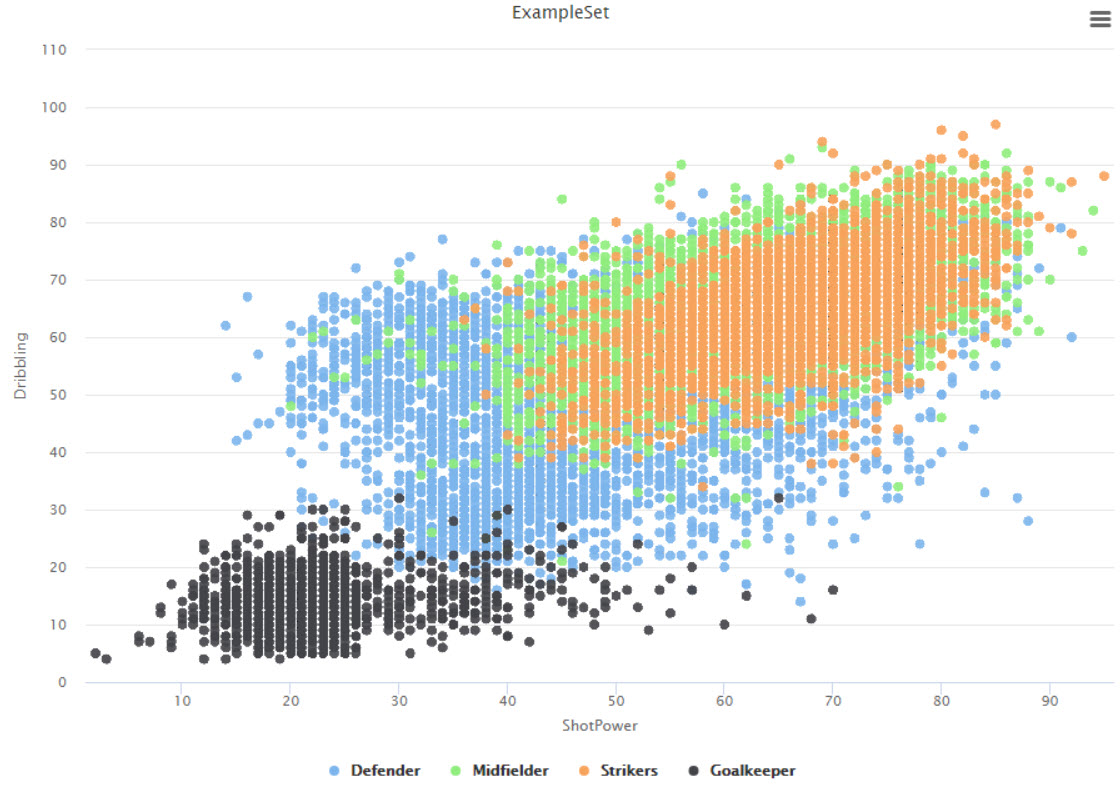
\includegraphics[width=8cm]{VisualizationAttributes.jpg}
  \caption{Visualization of two characteristics: dribbling and shot power}
  \label{fig:VisualAttributes}
\end{figure}

The result matches the expectations as the boundaries between strikers and midfielders are blurry. These two attributes are only an excerpt from more than 80 attributes but are typical for the data set.

As a conclusion, the data model to predict a soccer players position scores good result on the training and test data sets. Due to nearly identical attribute values for midfielders and strikers the accuracy decreased.












% ---- Bibliography ----
%
% BibTeX users should specify bibliography style 'splncs04'.
% References will then be sorted and formatted in the correct style.
%

\bibliographystyle{splncs04}
\bibliography{mybibliography}
%
\begin{thebibliography}{8}
%\bibitem{ref_article1}
%Author, F.: Article title. Journal \textbf{2}(5), 99--110 (2016)
%
%\bibitem{ref_lncs1}
%Author, F., Author, S.: Title of a proceedings paper. In: Editor,
%F., Editor, S. (eds.) CONFERENCE 2016, LNCS, vol. 9999, pp. 1--13.
%Springer, Heidelberg (2016). \doi{10.10007/1234567890}
%
%\bibitem{ref_book1}
%Author, F., Author, S., Author, T.: Book title. 2nd edn. Publisher,
%Location (1999)
%
%\bibitem{ref_proc1}
%Author, A.-B.: Contribution title. In: 9th International Proceedings
%on Proceedings, pp. 1--2. Publisher, Location (2010)
%
\bibitem{ref_rapidminergbt}
Rapidminer Documentation \url{https://docs.rapidminer.com/latest/studio/operators/modeling/\newline predictive/trees/gradient\_boosted\_trees.html}. Last accessed May 12, 2019
%
\bibitem{ref_sofifa}
Sofifa.com \url{https://sofifa.com/players}. Last accessed May, 12 2019
%\bibitem{ref_gitplayerstatistics}
%Sofifa.com \url{https://github.com/amanthedorkknight/fifa18-all-player-statistics/blob/master/README.md}. Last accessed May, 12 2019
\end{thebibliography}
\end{document}
